\documentclass{beamer}
\usepackage[ngerman]{babel}
\usepackage[utf8]{inputenc}
\usepackage[T1]{fontenc}
\usepackage{lmodern}

% bibliography
\usepackage{natbib}

% theme and colortheme
\usetheme{Berkeley}
\usecolortheme{spruce}
\setbeamertemplate{caption}[numbered]

% footer setting
\beamertemplatenavigationsymbolsempty
\setbeamertemplate{footline}[frame number]

% math mode settings
\usepackage{mathtools}
\usepackage{amssymb}
\usepackage{euler}
\usepackage[makeroom]{cancel}
\renewcommand{\deg}{\ensuremath{^{\circ}}}
\renewcommand{\epsilon}{\varepsilon}

% Grafikumgebungen
\usepackage{graphicx}
\usepackage{subcaption}
%\captionsetup[subfigure]{labelformat=parens, labelsep=quad}
\usepackage{floatflt}
\usepackage{float}

% table of contents at beginning of each section
%\AtBeginSection[]
%{
%  \begin{frame}
%    \frametitle{Contents}
%    \tableofcontents[currentsection]
%  \end{frame}
%}

% information to be included in the title page
\title{Bestimmung der Wolkenhöhe mittels Pyrgeometer}
\author{Lehrexkursion 2016 - Wolkenfernerkundung}
\date{\today}

%%%%%%%%%%%%%%%%%%%%%%%%%%%%%%%%%%%%%%%%%%%%%%%%%%
\begin{document}
\begin{frame}
\titlepage
\end{frame}

\section{Hintergrund}
\begin{frame}{Hintergrund}
\begin{columns}
\begin{column}{0.6\textwidth}
\begin{itemize}
  \vfill\item Bewölkung erhöht die langwellige Einstrahlung
  \vfill\item Die Strahlungsintensität hängt von der Temperatur des
      emittierenden Körpers ab \[ I \propto T\]
  \vfill\item Strahlungsmessungen enthalten Informationen über die
      Wolkentemperatur und ermöglichen so Rückschlüsse auf die Wolkenhöhe
  \vfill
\end{itemize}
\end{column}

\begin{column}{0.4\textwidth}
\begin{figure}[ht]
    \centering
    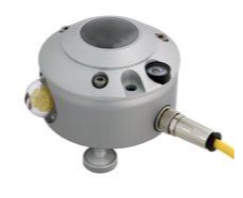
\includegraphics[width=1\textwidth]{figures/pyrgeometer.png}
    \caption{Pyrgeometer}
    \label{fig:pyrgeometer}
\end{figure}
\end{column}
\end{columns}
\end{frame}


\section{Pyrgeometer}
\begin{frame}{Pyrgeometer}
\begin{columns}
\begin{column}{0.6\textwidth}
\begin{itemize}
  \vfill\item Messung der atmosphärischen Gegenstrahlung $L\downarrow$\\
              (5 bis 50\,$\mu$m)
  \vfill\item Schwarze Sensoroberfläche mit Abschirmung der kurzwelligen
      Einstrahlung
  \vfill\item Langwellige Nettostrahlung wird durch Wärmeleitung in einer
      Thermosäule ausgeglichen
\vfill
\end{itemize}
\end{column}

\begin{column}{0.4\textwidth}
\begin{figure}[ht]
    \centering
    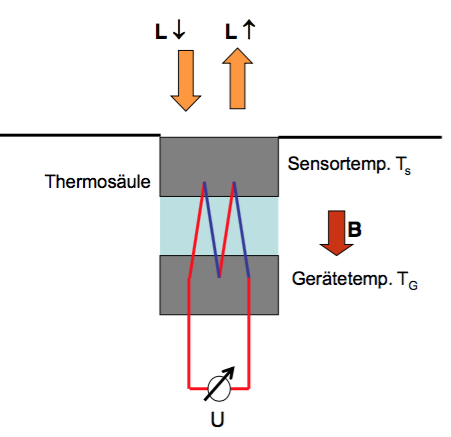
\includegraphics[width=1\textwidth]{figures/pyrgeometer_funktion.png}
    \caption{Aufbau}
    \label{fig:pyrgeometer_funktion}
\end{figure}
\end{column}
\end{columns}

\begin{alertblock}{Pyrgeometerformel}
  \centering$ L\downarrow = \lambda (T_S - T_G) + \sigma T_G^4 \approx cU + \sigma T_G^4 $
\end{alertblock}
\end{frame}


\section{Konzept}
\begin{frame}{Konzept}
\begin{itemize}
  \vfill\item Berechnung der Wolkentemperatur aus den Strahlungsmessungen des
      Pyrgeometers
  \vfill\item Zuordnung der Wolkentemperatur zu einer Höhe
  \begin{itemize}
    \item adiabatische Abnahme der Temperatur ausgehend\\
          von der Bodentemperatur $T_s$
    \item Standardatmosphäre mit angepasster $T_s$
    \item Radiosondenaufstieg
  \end{itemize}
  \vfill
\end{itemize}
\end{frame}


\section{Strah\-lungs\-trans\-fer}
\begin{frame}{Opazität}
\begin{columns}
\begin{column}{0.45\textwidth}
\begin{itemize}
  \vfill\item Großteil der gemessenen Strahlung entstammt der bodennahen Atmosphäre
  \vfill\item Optisches Fenster zwischen 20-40\,THz erlaubt Blick in höhere
      Atmosphärenschichten
  \vfill
\end{itemize}
\end{column}

\begin{column}{0.55\textwidth}
\begin{figure}[ht]
    \centering
    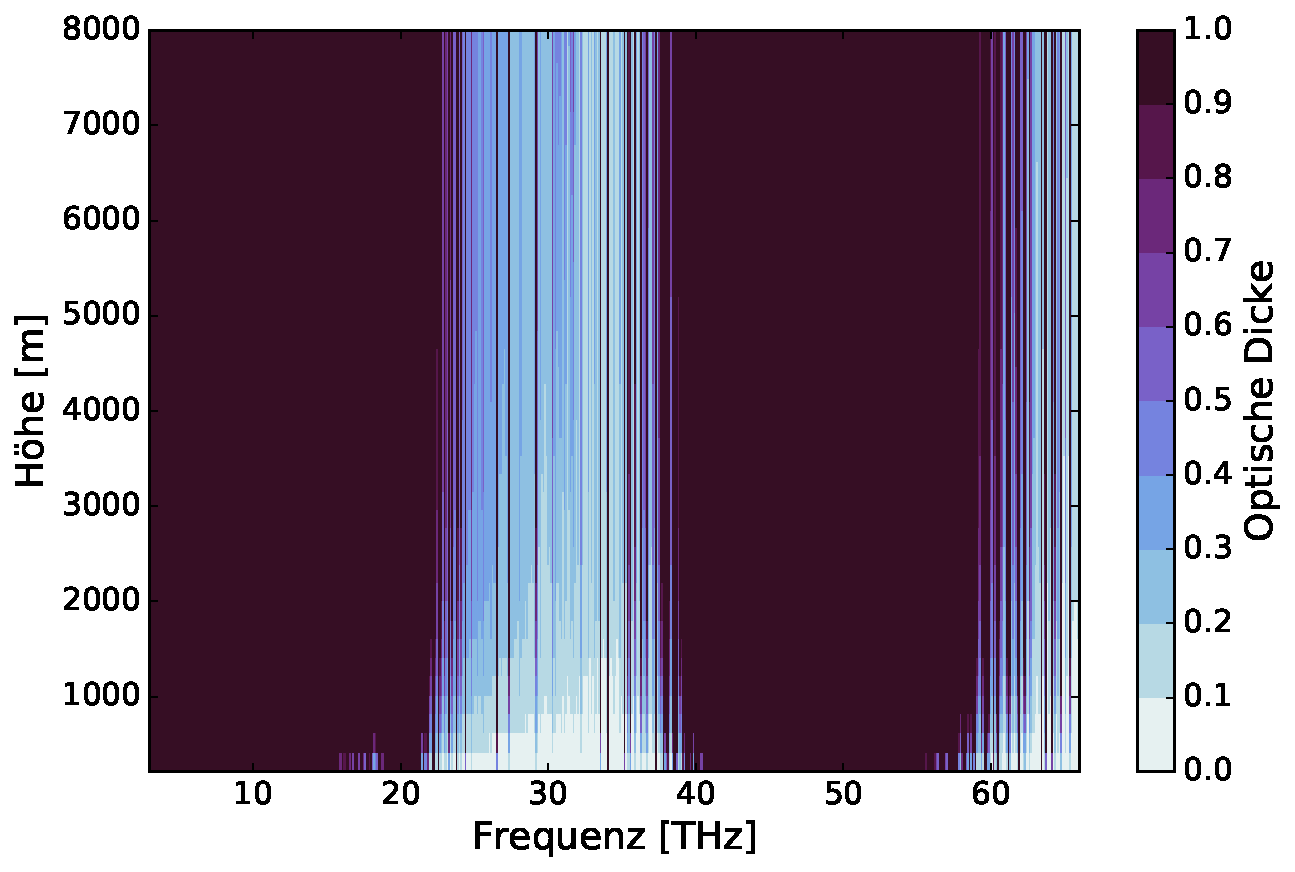
\includegraphics[width=1\textwidth]{figures/midlatitude-summer_window.pdf}
    \caption{Opazität in Abhängigkeit von Frequenz und Höhe.}
    \label{fig:window}
\end{figure}
\end{column}
\end{columns}
\end{frame}

\begin{frame}{Radianzspektrum}
\begin{figure}[ht]
    \centering
    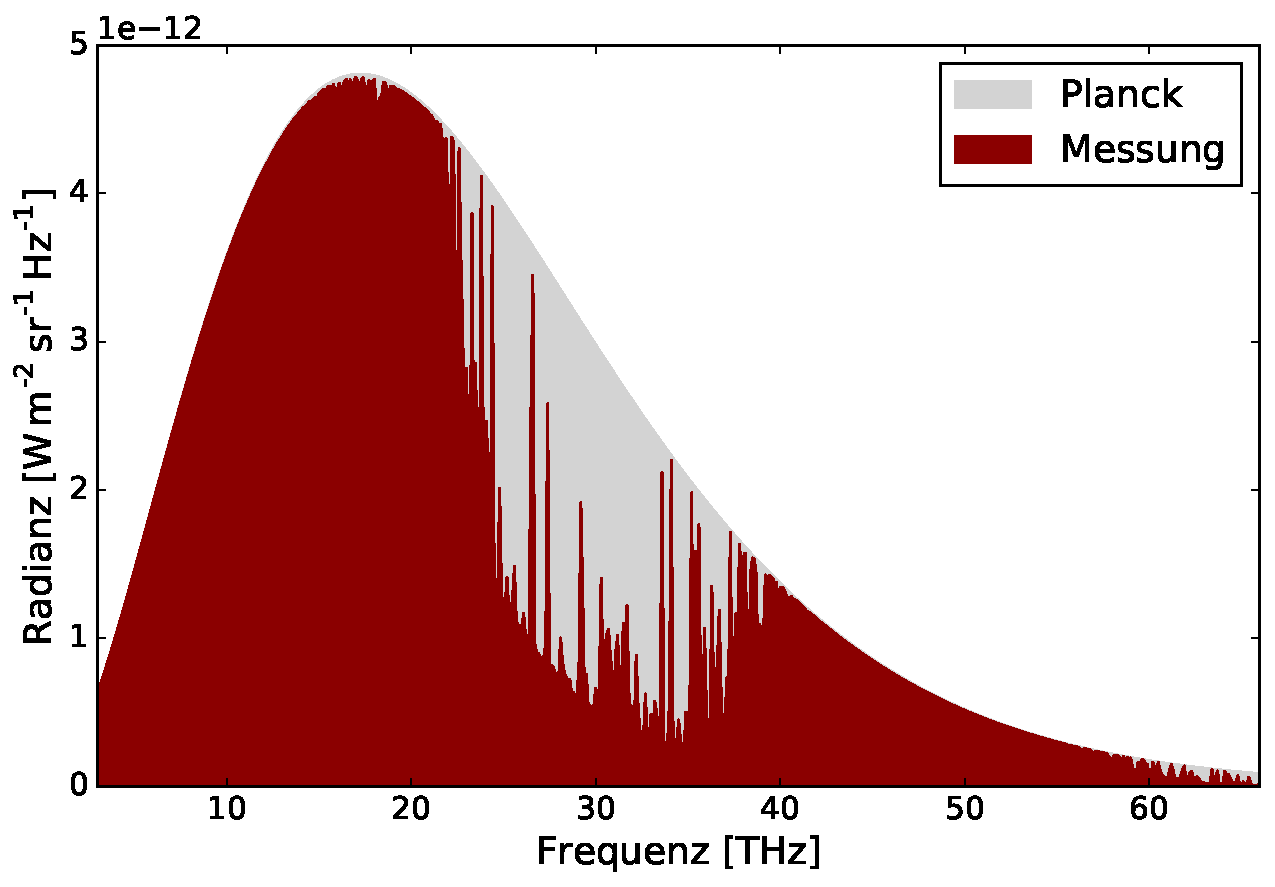
\includegraphics[width=0.8\textwidth]{figures/midlatitude-summer_spectrum.pdf}
    \caption{Radianz in Abhängigkeit der Frequenz.}
    \label{fig:spectrum}
\end{figure}
\end{frame}

\begin{frame}{Abschätzung der CLB}
\begin{itemize}
  \vfill\item Differenz der gemessenen LWR und der LWR der bodennahen
      Atmosphäre ist die entscheidende Größe
      \[ \Delta LWR = LWR - \int B_\nu(\nu, T_s) \partial\nu \]
  \vfill\item Die Differenz der Helligkeitstemperaturen $\Delta T_{LWR}$ gibt
      anschaulich an, wie viel Kelvin das optische Fenster kälter ist als die
      Temperatur am Boden
  \vfill\item Umrechnung in eine Höhe mittels Temperaturgradienten $\gamma$
      \[ CLB_{est} = \frac{\Delta T_{LWR}}{\gamma} \]
  \vfill
\end{itemize}
\end{frame}


\section{Ergebnisse}
\begin{frame}{Ergebnisse}
\begin{figure}[ht]
    \centering
    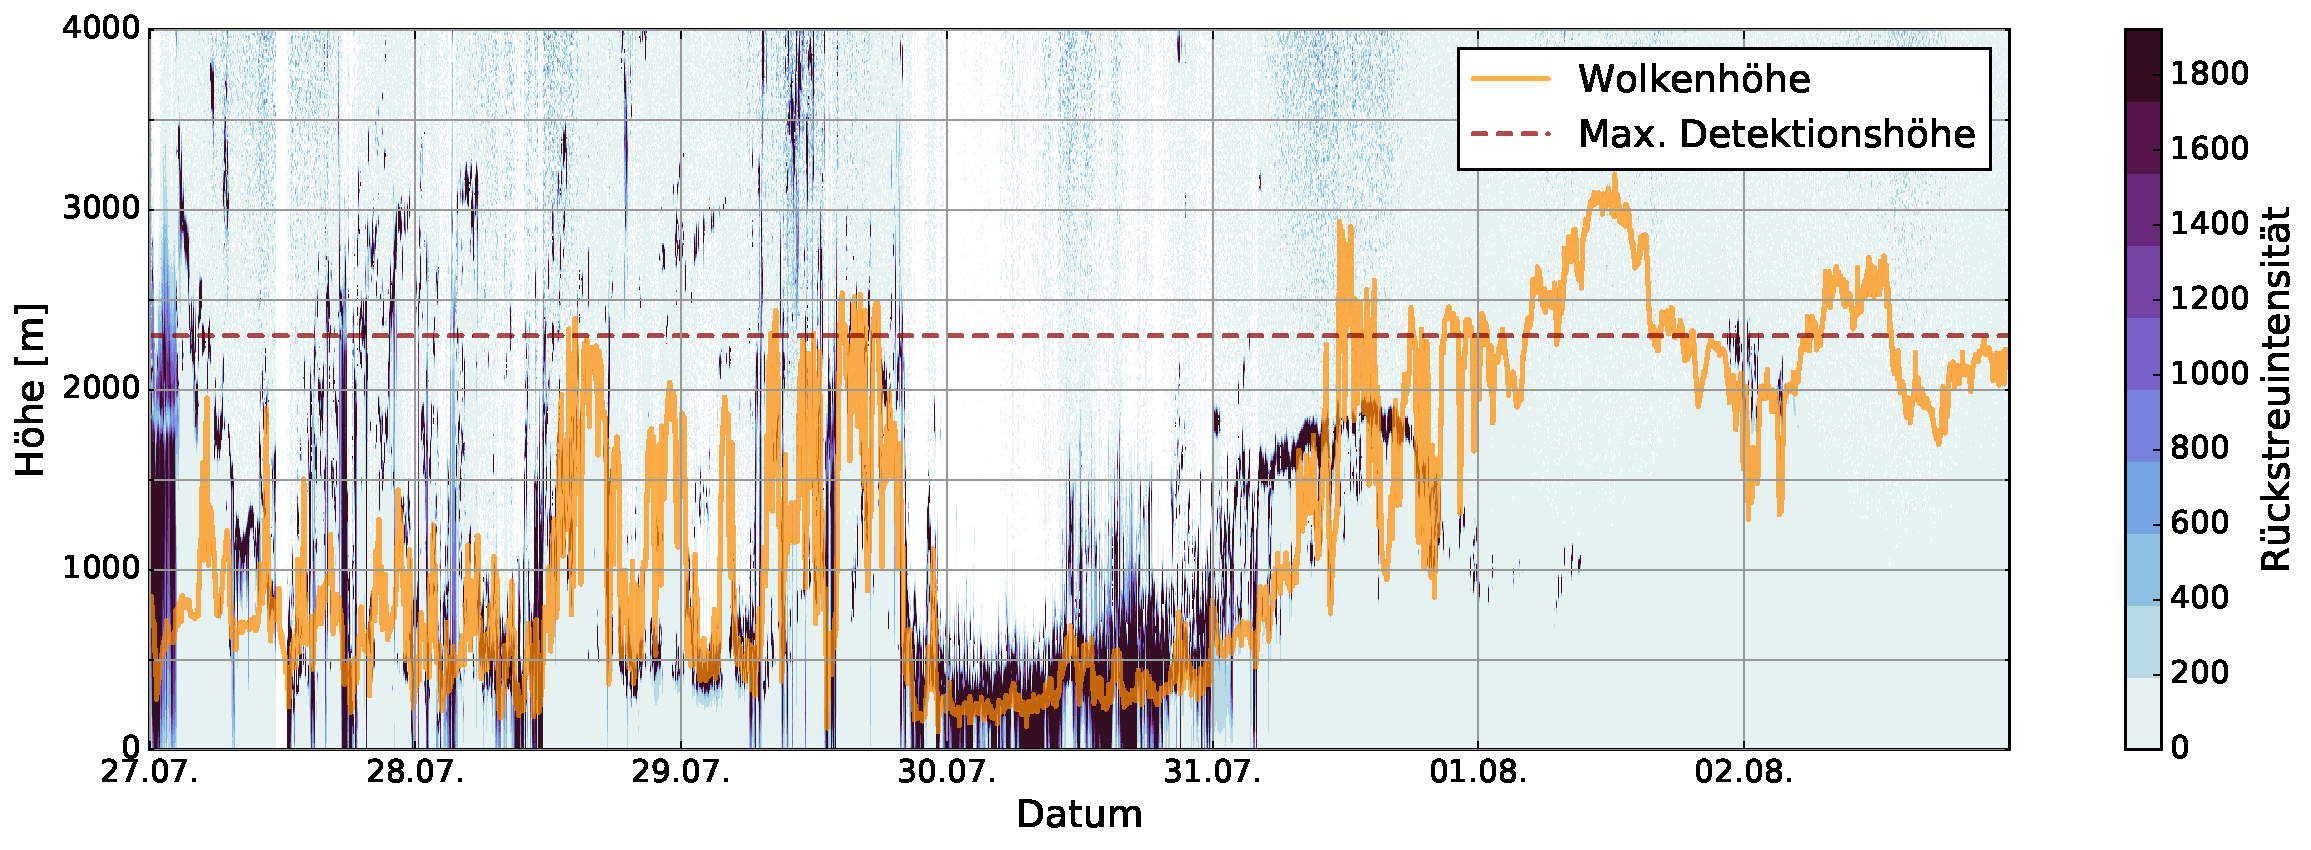
\includegraphics[width=1\textwidth]{figures/clb.pdf}
    \caption{Zeitreihe der berechneten Wolkenhöhe sowie der Ceilometer-Rückstreuung.}
    \label{fig:clb}
\end{figure}
\begin{itemize}
  \item $CLB_{est}$ im wolkenfreien Fall gibt eine Abschätzung der maximalen
      Detektionshöhe
\end{itemize}
\end{frame}

\begin{frame}{Fazit}
\begin{itemize}
  \vfill\item Messungen der langwelligen Gegenstrahlung und der bodennahen
      Temperatur (2\,m) ermöglichen eine Abschätzung der Höhe tiefer Bewölkung
  \vfill\item Die maximale Detektionshöhe hängt stark vom Atmosphärenzustand ab
      und liegt zwischen 2300 und 3500\,m
  \vfill\item Variabilität des vertikalen Temperaturgradienten kann die
      Ergebnisse verschlechtern 
\vfill
\end{itemize}
\end{frame}

\section{Ausblick}
\begin{frame}{Ausblick}
\begin{itemize}
  \vfill\item Verbesserung des vertikalen Temperaturgradienten über
      Einbeziehung der Bodenfeuchte
  \vfill\item Einschränkung des Pyrgeometer-Blickwinkels (Metallrohr) zur
      besseren Vergleichbarkeit mit Ceilometermessungen
  \vfill\item Wasserdampfretrieval an wolkenfreien Tagen
  \vfill
\end{itemize}
\end{frame}

\begin{frame}{Wasserdampfretrieval}
Wolkenfreie Messungen enthalten Informationen über den Wasserdampfgehalt der
Atmosphäre. Eine Regression von Strahlungstransfersimulationen verschiedener
Atmosphären bietet die Möglichkeit die Wasserdampfsäule abzuschätzen.

\begin{figure}[ht]
    \centering
    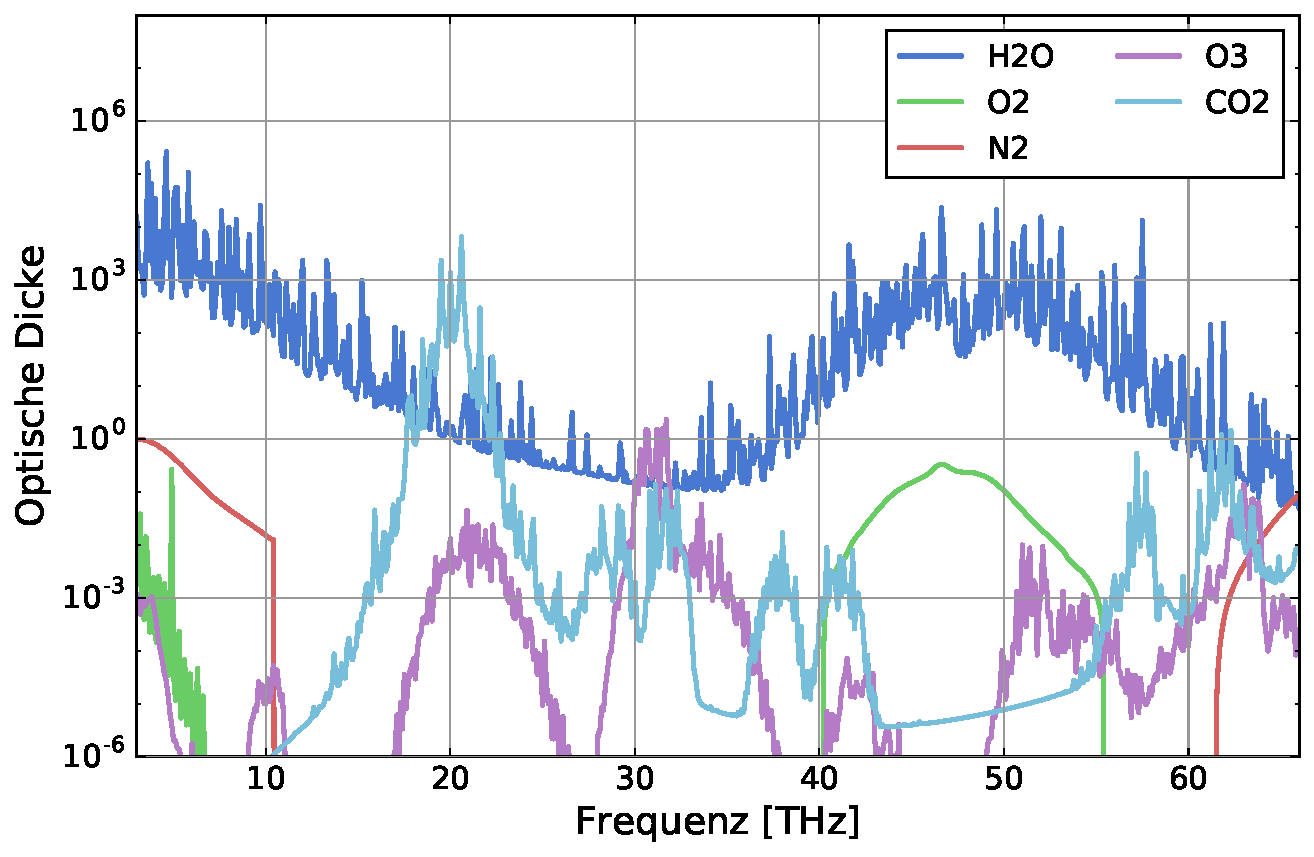
\includegraphics[width=0.7\textwidth]{figures/midlatitude-summer_opacity.pdf}
    \caption{Opazitätsspektrum verschiedener Absorber.}
    \label{fig:opacity}
\end{figure}
\end{frame}

\end{document}
